%*************************************************************
\chapter{Design VS Computer}\label{ch:DesignVSComputer}
%*************************************************************

Wir arbeiten mit Dokumenten in zwei verschiedenen Welten: der elektronischen Welt des Computers und der physikalischen Welt am Schreibtisch. Jede Welt hat Vorteile und Nachteile (siehe \autoref{tab:wellnerDokumente}), welche uns dazu bewegen die >>richtige<< für bestimmte Aufgaben zu wählen.

\begin{table}
    \myfloatalign
\begin{tabularx}{\textwidth}{p{5cm}X}
    \toprule
	    \tableheadline{Elektronische Dokumente} & \tableheadline{Papierdokumente}
	     \\ \midrule
		\begin{itemize} 
			\item{schnell zum editieren}
			\item{schnelles kopieren}
			\item{schnelles senden}
			\item{schnelles freigeben}
			\item{schnelles ablegen}
			\item{schnelles abrufen}
			\item{erlaubt Stichwortsuche}
			\item{erlaubt \newline Rechtschreibprüfung}
			\item{erlaubt sofortige \newline Berechnungen}
		\end{itemize} &
		\begin{itemize} 
			\item{3-dimensional}
			\item{überall akzeptiert}
			\item{billig}
			\item{portabel}
			\item{geläufig}
			\item{hochauflösend}
			\item{einfach zu lesen}
			\item{fühlbar}
			\item{man kann beide \newline Hände \& Finger \newline zum bearbeiten \newline verwenden}
			\item{man kann mit einem Stift darauf kritzeln}	
		\end{itemize}
	\\  \bottomrule
\end{tabularx}
  \caption[Elektronische Dokumente und Papierdokumente]{Gegenüberstellung der Eigenschaften von elektronischen Dokumenten und Papierdokumenten.}
  \label{tab:wellnerDokumente}
\end{table}

\medskip In mancher Hinsicht scheint es aber, als wäre Papier bald obsolet. Manche prophezeien das papierlose Büro schon in wenigen Jahren. Das Eigenartige dabei ist nur, dass sich die Leute ungern von Papier trennen. Studien belegen, dass der Papierkonsum in Büros seit 1970 um das 6-fache anstieg und derzeit jährlich um 20\% steigt \citep{seybold:1992}. Papier hat ebenso wie elektronische Dokumente Eigenschaften, die Menschen nicht aufgeben wollen. Das macht sie in Hinsicht auf computerbasierende Alternativen >>unverwüstlich<<. \citep{Luff:1992} 

\medskip Wie wichtig Papier (im Zusammenhang mit Skizzen) für Designer ist, wurde auch im Kapitel \nameref{ch:designTheorie} beschrieben. Welchen Umstand dies das alte Medium zu verdanken hat, lässt sich laut Sellen und Harpers Arbeit \emph{The Myth of the Paperless Office} \citep{Sellen:2003} nicht durch einfache Merkmalgegenüberstellungen herausfinden. Nur Studien und Observationen können das kognitive Verhalten bei der Benutzung von Papier und digitalen Artefakten beschreiben. 

\medskip Das nun folgende Kapitel soll die Stärken und Schwächen traditioneller und digitaler Arbeitsweisen gegenüberstellen und mittels verschiedenster Studien eine Erklärung zum oben genannten Phänomen finden. -- Können die beiden Welten von einander lernen?
%Deswegen initierten Terrenghi et al. eine Designstudie, die dabei helfen sollte, das kognitive Verhalten bei der Benutzung von Papier und digitalen Artefakten zu beschreiben. \citep(Terrenghi:2007) Ihre Ergebnisse sollen in den nächsten beiden Abschnitten erläutert werden.

\section{Skizzieren auf Papier}
%Skizzieren erlaubt Personen mit abstrakten und ungenauen Elementen zu arbeiten, diese daraus resultierenden oft mehrdeutigen Kritzeleien wiederholt zu interpretieren und alternative Bedeutungen zu erlangen. Skizzierte Abbildungen, Bilder und Karten helfen Personen ihre Gedanken zu manifestieren oder Ideen anderen zu erklären. \citep{YiLuenDo:2005}
Skizzieren fördert eine schnelle und formlose Informationsverarbeitung. Wir würden z.B. eine Telefonnummer eher auf ein Whiteboard in der Nähe des Schreibtischs schreiben, als sie in den Computer einzugeben; bzw. schnelle Berechnungen oder \emph{To-Do-Lists} auf einem Blatt Papier, da sie leicht zu erstellen sind und das Ergebnis portabel ist.
Larkin und Simon verglichen \emph{schematische} Darstellungen mit \emph{Darstellungen in der Wortebene} (geschrieben oder gesprochen) und zeigen damit dass räumliche Darstellungen oft mehr aussagen als die gleiche Information in einem ausführlich geschriebenen Statement \citep{Larkin:1987}. Wie effizient Information verarbeitet werden kann hängt - technisch betrachtet - davon ab wieviel >>Rechenaufwand<< von Nöten ist, um Vorgaben so zu übersetzen damit Verständnis entsteht. Um beispielsweise einen mathematischen Ausdruck eines Verhältnisses zu beschreiben, würde sich eine schematische Darstellung besser eignen. Der gleiche Ausdruck als Darstellung in der Wortebene würde eine längere Berechnungszeit benötigen (vgl. \autoref{fig:johnsonDarstellungsformen}).

\begin{figure}
        \myfloatalign
        \subfloat[Geschriebene Darstellung (in der Wortebene).]
        {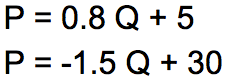
\includegraphics[width=.48\linewidth]{gfx/johnsonDarstellungsformenB}} \quad
        \subfloat[Graphische (schematische) Darstellung.]
        {\label{fig:basteaEvaluationSketchingInput}%
         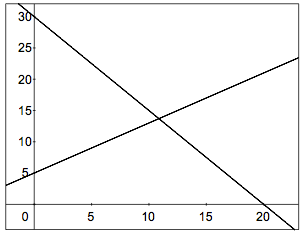
\includegraphics[width=.48\linewidth]{gfx/johnsonDarstellungsformen}} \\
        \caption[Darstellungsformen]{Die schematische Darstellung (a) und die Darstellung in der Wortebene (b) eines mathematischen Verhältnisses. Beide Darstellungsformen zeigen die gleiche Information. }\label{fig:johnsonDarstellungsformen}
\end{figure}

\medskip Wenn Personen skizzieren, fassen sie relevante Informationen zusammen und lassen die irrelevanten aus \citep{Tversky:2002}. Zeichnen erlaubt Personen Papier als externen Speicher zu verwenden, um ihre kognitive Belastung zu verringern. Schematische Darstellungen stellen ein vereinfachtes Abbild von Informationsbereichen dar \citep{Tversky:2000}. Per Hand gezeichnete Landkarten bzw. Wegbeschreibungen zum Beispiel, werden üblicherweise mit simplen Formen wie Rechtecke oder Kreise für Gebäude, Linien oder Pfeile für Wege und sich überschneidende Linien für Kreuzungen gezeichnet \citep{Tversky:1999}. Die Form und Krümmung von Gebäuden und Linien werden lediglich geschätzt. Bei einer gut gezeichneten Karte hingegen haben Menschen Schwierigkeiten die kleinen Unterschiede zwischen der Karte und der echten Welt abzugleichen. Räumliche Darstellungen sind ebenso ein beeindruckendes Hilfsmittel beim Lernen. Skizzieren erlaubt Lernenden Konzepte, so wie sie verstanden wurden, aufzuzeichnen und diese von erfahrenen Personen auf Inkonsistenzen und Fehlern zu überprüfen \citep{Forbus:2008}.
%Van Sommers studierte ausgiebig das Zeicheinverhalten von Personen \citep{VanSommers:1984}. 

\medskip \citeauthor{Goel:1995} führte eine Reihe an Experimenten durch, um die kognitiven, handlungsauffordenrnden Merkmale von Skizzen zu erforschen. In seinen Studien verglich er traditionelle Papier-und-Stift Skizzen mit Skizzen, die mit Hilfe von computerbasierten Zeichenprogrammen erstellt wurden. Die teilnehmenden Designer bekamen Anweisungen ein Artefakt auf beide Arten zu designen. Dabei kam ein modifiziertes Softwaretool zum Einsatz, das lediglich strukturierte Eingaben, wie gerade Linien, Rechtecke und Ellipsen unterstützte. Die Ergebnisse zeigten, dass das strukturierte Computerprogramm bezüglich der Ideenfindung, nicht an die Schnelligkeit vom unstrukturierten Papier-und-Stift System herankam. Skizzieren unterstützt Designer bei der schnellen Entwicklung vieler unterschiedlicher Ideen. Diesen explorativen Charakter von Skizzen beschrieb Goel als \emph{Quertransformationen}, die sich im Gegensatz zu den \emph{vertikalen Transformationen}, welche sich durch Verfeinern von Ideen auszeichnen, deutlich abgrenzen. Bei den beiden Transformationstypen stützt sich Goel auf die von Newman und Landay in \citep{Newman:2000} beschriebenen Aktivitäten verschiedener Designstufen. Am Anfang des Designprozesses sind Designer mit der Ideengenerierung und -findung beschäftigt (Quertransformationen). Später konzentrieren sich Designer schrittweise Überarbeitungen und Änderungen (vertikale Transformationen).

\medskip 

\section{Skizzieren am Computer}

Heutige stiftbasierte Hardware orientiert sich vorwiegend am Schreiben und Lesen von Text. Wenn man erwägt diese auch für Designaktivitäten einzusetzen, sollte man sie mit den Werkzeugen, die Designer in der Praxis benutzen vergleichen. \\ Designer können schnell Zeichnungen auf Papier anfertigen und zwischen den einzelnen Seiten blättern. Sie können ebenfalls die Zeichnungen nebeneinander an die Wand heften, um sie zu vergleichen. Die Stiftspitze zeichnet dabei sofort bei Berührung auf dem Papier und es können zwei Hände benutzt werden um das Blatt Papier nach Belieben zu drehen bzw. um Hilfsmittel wie ein Lineal zu halten.

\medskip Am einfachsten wäre es, wenn computerunterstützes Skizzieren genau die selben Eigenschaften aufweisen würde. Jedoch mangelt es der derzeitigen Hardware an Portabilität, schnellem Reaktionsvermögen und dem vertrauten Gefühl traditioneller Designpraktiken. Die kommerzielle Entwicklung und Forschung verbessert kontinuierlich Hardware auf diesem Sektor, so unterstützen viele Geräte wie z.B. PDAs, Tablet PCs oder interaktive Wandinstallationen bereits eine Art von Stift- oder Touchinput. Während stiftbasierte Systeme seit Jahrzehnten bei Forscher im Einsatz sind, verbreiten sie sich erst seit Mitte der 90er Jahre und werden stetig billiger.

\medskip >>Skizzierhardware<< kann in zwei Gruppen unterteilt werden: 
\begin{itemize}
	\item{Hardware, die nur Eingaben unterstützt, und}
	\item{Hardware, die Eingaben und Ausgaben unterstützt.}
\end{itemize}

Tablets geben den Benutzern die Möglichkeit mit Hilfe eines Eingabestifts zu schreiben bzw. zu zeichnen. Manche beschränken sich dabei aber lediglich auf die Eingabe und zeigen nicht gleichzeitig das Gezeichnete. Geräte, die Ein- und Ausgaben unterstützen, haben sich besonders bei den Tablet PCs durchgesetzt. Zusätzlich gibt es auch Systeme, die das gezeichnete indirekt >>scannen<<. Z.B. entwickelte PARC das ScanScribe System, welches Zeichnungen analysiert, die mit herkömmlichen Stift und Papier erzeugt wurden und erstellt daraus eine mit dem Computer aufgebesserte Version. \citep{Johnson:2009}

\subsection{Electronic Ink}
Wenn man eine Zeichnung mit künstlerischem Ausdruck zu Papier bringt, gibt es viele Faktoren die das Endergebnis beeinflussen. So z.B. die Stärke des Schreib- bzw. Zeichengeräts, sowie die Materialeigenschaften des Papiers. In vielen Branchen, wie beispielsweise in der Computeranimation, ist es noch immer üblich Illustrationen zuerst auf Papier zu zeichnen und danach schrittweise zu digitalisieren. Es wurden zwar einige Versuche gestartet direkt auf digitaler Ebene zu zeichnen, jedoch wird dies nach wie vor hauptsächlich nur dort verwendet, wo der Computer nicht nur optional benutzt wird. \citep{Henzen:2005}

Viele Tablets sind Druckempfindlich. Designer benutzen oft stärkere Linien um Objektgrenzen hervorzuheben und dünne Linien um dezente Texturen, Schatten oder Rundungen anzudeuten. Geräte, die Druck messen können, erlauben Designer dickere oder dunklere Striche zu zeichnen, ohne vorher in einen anderen Zeichenmodus wechseln zu müssen.

Die Druckmessung wurde auf verschiedene Weisen umgesetzt. Z.B. durch zwei übereinander liegenden leitfähigen Schichten mit entgegengesetzten Stromrichtungen. Die Schichten berühren sich nicht und sind oft durch eine nicht leitende Flüssigkeit abgeschirmt. Wenn etwas (ein Stift oder Finger) die obere Schicht berührt, verändert sich die Spannung und die Position kann mittels Interpolation an den Kanten errechnet werden. Andere berührungsempfindlichen Oberflächen messen die elektrischen Eigenschaften der Dinge, die sie berühren -- darum funktionieren auch Handschuhe auf manchen Laptop Trackpads nicht. Wacom\texttrademark{} Tablets und gleichartige induktive Geräte, benötigen spezielle Stifte, die in einem vom Tablet generierten elektromagnetischen Feld mitschwingen. Wieder andere Tablets erkennen akkustische oder optische Störungen zur Positionsberechnung.

Es gibt Oberflächen, die lediglich die Koordinaten eines einzigen Berührungsortes liefern können und Oberflächen die mehrere erkennen - auch Multitouchoberflächen genannt. Multitouchsysteme, wie z.B. \emph{Hans's Frustrated Total Internal Reflection technique} \citep{Han:2005} und \emph{Microsoft's Surface System} \citep{Surface:2010} befinden sich derzeit im Aufschwung, werden aber mit den Fingern order Händen benutzt und bieten deswegen völlig andere Anwendungserlebnisse als Stiftbasierte Oberflächen.

\subsection{Der Unterschied zwischen Eingabestift und Maus}

Egal welche Abtasttechnologie man wählt, alle oben genannten Geräte erlauben Benutzern eine Eingabevariante, die näher an das traditionelle Schreiben herankommt, als die Maus jemals könnte. Obwohl Stift- und Mauseingaben viele Eigenschaften teilen (beide erlauben Benutzer im 2D Raum zu interagieren), haben sie einige grundlegende Unterschiede.

\medskip Mauseingaben liefern Daten über die \emph{Bewegung} - und Stifteingaben liefern Daten über die \emph{Position} \citep{Hinckley:2002}. Mit anderen Worten produzieren Mäuse relative \emph{Änderungen} in der (x,y) Position und Stifte direkte, absolute (x,y) Positionen. Benutzer können Tablets aber auch so konfigurieren, damit sie sich wie Mäuse verhalten und relative Positionen erzeugen.

\medskip Die Form der Geräte ist ebenfalls extrem wichtig. Ein Stift zwingt die Benutzer die Feinmotorik ihrer Finger einzusetzen um die Stiftspitze zu steuern, wohingegen die Hand- und Unterarmmuskeln die Maus steuern. Finger können zwar auch zur Maussteuerung benutzt werden, aber nicht mit der gleichen Fertigkeit. Je nach Art der Arbeit, ist ein Stift ergonomisch besser als eine Maus - oder umgekehrt.

Tablets können aber mehr als nur die Stiftposition erkennen. Manche Geräte können auch den Aufpressdruck, den Winkel oder die Rotation des Stifts messen. Das andere Ende des Stifts wird auch oft als alternativer Modus (z.B. als ein Radierer) benutzt. 

Einige Stifte haben noch zusätzliche Buttons. Während Buttons unentbehrliche Bestandteile von Mäusen sind, können sie entlang des Stiftgehäuses schwer benutzbar sein \citep{Plimmer:2008}. Die Kraft, die bei einem Buttonklick an der \emph{Maus} entsteht, ist orthogonal zu der Oberfläche, auf der die Maus benutzt wird und beeinflusst die Zielgenauigkeit nur unwesentlich. Ein Knopfdruck am \emph{Stift} hingegen, kann die Stiftspitze ungewollt bewegen, was das Zeigen auf ein bestimmtes Objekt und das gleichzeitige Drücken einer Taste erschwert (siehe \autoref{fig:johnsonButtonPress}). Zudem muss der Benutzer beim Drücken einer Taste üblicherweise den Stift erst so drehen, damit sich sein Finger wieder über der Taste befindet (was durchaus öfter vorkommt). Diese Aktion lenkt ab und ist auf längere Zeit gesehen unbequem. \citep{Johnson:2009}

\begin{figure}
        \myfloatalign
        \subfloat[Drücken einer Maustaste erzeugt eine Kraft, die orthogonal auf die darunterliegende Oberfläche wirkt.]
        {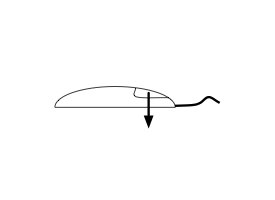
\includegraphics[width=.48\linewidth]{gfx/johnsonMousePress}} \quad
        \subfloat[Drücken einer Stifttaste erzeugt eine ungewollte Stiftspitzenbewegung.]
        {\label{fig:johnsonButtonPressB}%
         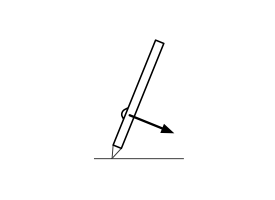
\includegraphics[width=.48\linewidth]{gfx/johnsonStylusPress}} \\
        \caption[Kräfte bei Buttonklicks.]{Entstehende Kräfte beim Drücken einer Maustaste (a) und einer Stifttaste (b) eines Tablets.}\label{fig:johnsonButtonPress}
\end{figure}

\subsection{Interaktionstechniken für stiftbasierte Skizziersysteme} %5.5
Bei der Entwicklung neuer Technologien ist es wichtig das Ausmaß der kognitiven Belastung des Tools zu berücksichtigen. Aus Oviatt's Studie \citep{Oviatt:2006} über Mathematikstudenten geht hervor, dass das Arbeiten mit stiftbasierte Applikationen auf Tablet PCs erheblich schlechter funktioniert als mit herkömmlichen Stift und Papier. Durch die Benutzung der Tablets benötigten die Studenten mehr Zeit bei der Lösung von Mathematikaufgaben, was dazu führte dass sie sich mit der Technologie nicht anfreunden konnten. Anthony et al. führten eine ähnliche Studie durch, in der sie Eingaben von Studenten verglichen, die Gleichungen beinhalteten. Zur Eingabe dienten ein \emph{Standard WIMP\footnote{Die Abkürzung WIMP wurde 1980 von Merzouga Wilberts ins Leben gerufen und steht für Window, Icon, Menu, Pointing Device. Es bezeichnet das Grundkonzept moderner grafischen Benutzerschnittstellen (GUIs).} Interface} und ein Eingabetablet \citep{Anthony:2005}. \\ Sie kamen zur Erkenntnis, dass die Studenten Stifteingaben bevorzugten und handgeschriebene Gleichungen schneller und genauer niederschreiben konnten, als mit Keyboard und Maus. Papier und Stift wurden dem elektronischen Schreiben zwar vorgezogen, jedoch waren ihnen Stifte im Allgemeinen lieber als Tastatur- und Mauseingaben. Beide Studien kamen zum selben Schluss: Je mehr Aufmerksamkeit Benutzer aufbringen müssen um das Tool zu verwenden, desto weniger Aufmerksamkeit schenken sie dem eigentlichen Problem.

\medskip Zur Redzuierung der kognitiven Belastung müssen demnach natürlichere Interaktionstechniken entwickelt werden. Verschiedenste Methoden erwiesen sich bis dato durchaus brauchbar zum effizienten Arbeiten mit Stiftapplikationen. Kontextmenüs sind ein gutes Beispiel dafür \citep{Kurtenbach:1991}. Traditionelle Menüs zeigen eine Liste an Optionen, welche das Menü nach unten und rechts wachsen lassen. Bei Tablets, die Eingaben und Ausgaben unterstützen (z.B. Tablet PCs) kann dies dazu führen, dass Benutzer das Menü mit der Hand verdecken. >>Torten<<-Menüs (eine Art Kontextmenü) erscheinen zentriert um die Stiftposition und zeigen die Optionen kreisförmig (siehe \autoref{fig:johnsonPieMenu}). Die Hand ist zwar bei dieser Art von Menüs noch immer teilweise im Weg, aber zumindest ist ein Teil des Menüs dadurch sichtbar. Der Vorteil dieser Methode ist, dass sich Personen Gesten anlernen können, ohne die Menüeinträge jedesmal erneut lesen zu müssen. Vorraussetzung dafür ist jedoch, dass sich die Menüeinträge niemals ändern. Eventuell schwindet auch der Bedarf eines visuellen Menüs durch die Gesten. Tortenmenüs werden in Applikationen wie Maya \citep{Maya:2010}, Spielen wie The Sims \citep{EA:2010} oder als Erweiterungen in Webbrowser verwendet. Der Ansatz funktioniert zwar gut, bringt aber auch zwei Nachteile mit sich. Zum einen ist es nicht klar wie man das Menü aufrufen kann und zum anderen müssen Gesten erst entdeckt, erlernt und ins Gedächtnis gerufen werden.

\begin{figure}
        \myfloatalign
        \subfloat[Tortenmenüerweiterung für den Firefox Webbrowser.]
        {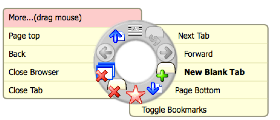
\includegraphics[width=.48\linewidth]{gfx/johnsonPieMenuFF}} \quad
        \subfloat[Autodesk Maya Tortenmenü.]
        {\label{fig:johnsonPieMenuB}%
         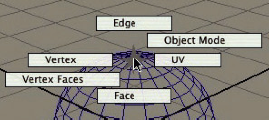
\includegraphics[width=.48\linewidth]{gfx/johnsonPieMenuMaya}} \\
        \caption[Tortenmenüs]{Tortenmenüs in Firefox (a) und Maya (b).}\label{fig:johnsonPieMenu}
\end{figure}

\medskip Ramos et al. \citep{Ramos:2004} erforschte weiters die Benutzung von Aufpressdruckdaten bei stiftbasierenden Interaktionen. Zu der zweidimensionalen (x,y) Stiftposition kommt die Druckstärke des Stiftes als dritte Dimension hinzu, die der Benutzer frei verändern kann. Zum Beispiel kann ein leichter Druck ein Menü zeigen und ein harter Druck ein anderes Menü. Druck kann eine effektive Eingabeart sein, wenn sie richtig (mit haptischen und visuellen Feedback) eingesetzt wird.

\medskip Hinckley et al. \citep{Hinckley:2005} empfiehlt die Benutzung von \emph{Begrenzer} um Kontextmenüs aufzurufen. \emph{Begrenzer} sind Eingaben, die Benutzer normalerweise nicht zeichnen würden aber dennoch leicht zu merken sind. Ein Beispiel zeigt ihr System Scriboli, in dem ein >>Rattenschwanz<< (eine Schleife am Ende einer Selektionsgeste) als Begrenzer benutzt wird. Diese flüssige Bewegung lässt den Benutzer Zielobjekte kennzeichnen um auf sie anschließend ein Kommando anwenden zu können.

\medskip Wieder andere haben Interface Idiome\footnote{siehe \nameref{sec:designPatterns}} zur Unterstützung von Stift- \& Skizzeneingaben entwickelt. \emph{Gedrics} sind auf Gesten basierende Icons für stiftbasierte Applikationen \citep{Geissler:1995}. Jedes Gedric ist mit einer Klasse an Aufgaben, wie >>ändere die Schriftarteigenschaften<< in einem Texteditor, verknüpft. Um ein Kommando durchzuführen, muss der Benutzer eine Geste auf ein Gedric zeichnen. Das System erkennt die Geste und gibt dem Icon anschließend die auf die Geste verknüpfte Bedeutung, welche durch Darauftippen aktiviert wird. Zeichnet man z.B. eine schräge Linie auf einem >>Schriftart<<-Gedric stellt das System einen markierten Text kursiv. Zeichnet man eine vertikale Linie von unten nach oben, wird die Schriftgröße erhöht. \\ So komfortabel Operationen auf Gedrics auch wirken, erfordern sie trotzdem eine Eingewöhnungsphase, in der Benutzer lernen müssen ihre Absichten in Gesten umzuwandeln. (vgl. \autoref{fig:geisslerGedric}) 

\begin{figure}
        \myfloatalign
        \subfloat[Gedric Icons.]
        {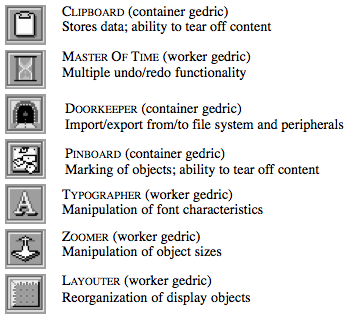
\includegraphics[width=.38\linewidth]{gfx/geisslerGedricIcons}} \quad
        \subfloat[Layouter Gesten.]
        {\label{fig:geisslerGedricIcons}%
         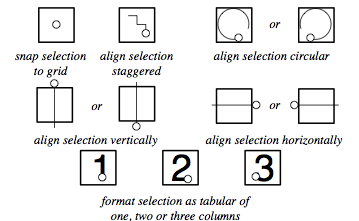
\includegraphics[width=.58\linewidth]{gfx/geisslerGedricLayouter}} \\
        \caption[Gedric]{Beispiele für Gedric Icons (a) und Gesten einer Layoutfunktion (b).}\label{fig:geisslerGedric}
\end{figure}

\medskip Während Point \& Click Aktionen für Aufgaben zu Anwendungen, die üblicherweise mit der Maus ausgeführt werden ausgelegt sind, raten Accot und Zhai zur \emph{Kreuzen}-Technik zur Stiftinteraktion \citep{Accot:2002}. Das experimentelle Zeichenprogramm \emph{CrossY} \citep{Apitz:2004} zeigt Interface Widgets\footnote{Widgets (dt. Steuerelemente) sind Interaktionselemente in einer grafischen Benutzeroberfläche (GUI), beispielsweise eine Schaltfläche oder eine Bildlaufleiste.}, die Kreuzen erlauben. Um ein CrossY Button zu aktivieren, muss der Benutzer eine Linie von einer Seite des Buttons zur anderen zeichnen, und somit den Button überqueren. Kreuzen macht es möglich mehrere Aktionen in einer flüssigen Bewegung abzuhandeln. Zum Beispiel kann man die Farbe und Stärke der Electronic Ink des Stiftes gleichzeitig ändern, in dem man den Stift über benachbarte CrossY Widgets bewegt (siehe \autoref{fig:accotCrossY}).

\begin{figure}[bth]
	\begin{center}
	
	{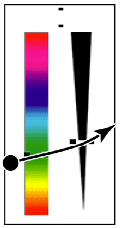
\includegraphics[width=0.3\linewidth]{gfx/accotCrossY}}
	\caption[CrossY]{CrossY Interface Widgets erlauben Benutzer mehrere Parameter mit einer einzigen Bewegung zu ändern -- in diesem Beispiel die Stiftfarbe und -stärke.}
	\label{fig:accotCrossY}
	\end{center}
\end{figure}

\medskip So wie Skizzen mehrdeutig sein können, können auch stiftbasierte Interaktionen, wie das Drücken eines Buttons oder die Auswahl eines Menüpunktes, mehrdeutig sein. Wenn der Benutzer mit Hilfe des Stiftes, mit einem Objekt interagieren will, kann es sein, dass das System sein Ziel erst eindeutig machen muss. Zum Beispiel kann beim Drücken eines Buttons der Stift unabsichtlich zu einem anderen Button rutschen. Dieser Umstand wird auch \emph{Target Amibiguity}, oder laienhaft übersetzt \emph{Ziel Mehrdeutigkeit} genannt \citep{Mankoff:2000p77} \citep{Mankoff:2000}. \\
Eine Alternative um gegen die Mehrdeutigkeit vorzugehen, ist sie im Voraus zu bekämpfen. Pegasus und Chateau demonstrieren in \citep{Igarashi:2001} und \citep{Igarashi:2003} ein \emph{Empfehlungssystem}, das vorhersagt was der Benutzer zeichnen wird und alle möglichen Aktionen aufzeigt. Diese Technik eignet sich besonders, wenn die Umgebung eine regelmäßige Grammatik aufweist oder strukturierte Eigenschaften wie Symmetrie genutzt werden soll.
Tsang et al. benutzten ein Empfehlungssystem in ihrem Programm, das Formen wie Flugzeugaußenhüllen modellieren kann \citep{Tsang:2004}. Das System bietet ein Overlay, das den Benutzer durch zusätzlichen Skizzierinput leitet. Benutzer zufolge führt dies zu präziseren Input. Das System benutzt die angefangenen Skizzen als Vorlagen, vergleicht diese mit Datenbankeinträgen um ähnliche Zeichnungen zu finden und empfielt zusätzliche Geometrie, die vielleicht dazu passen könnte.

\medskip Bae's 3D Kurvenmodellierungsystem zeigt wie verschiedene kaligraphische Interaktionstechniken zusammen benutzt werden können um eine flüssige Skizzierumgebung zu schaffen \citep{Bae:2008}. Das sog. \emph{ILoveSketch} System imitiert ein physikalisches Skizzierbuch. Die Eingaben erfolgen per Stift und können optional durch drücken von physikalischen Buttons durch die andere Hand verändert werden (siehe \autoref{fig:baeILoveSketch}). Das Interface verzichtet auf herkömmliche on-screen Buttons, Scrollbars und Menüs. Stattdessen gibt der Benutzer Kommandos durch Gesten, die oft vom Kontext abhängen. Zum Beispiel kann der Benutzer zu älteren Zeichnungen zurück >>blättern<<, in dem er an einer Ecke zieht. Um ein Objekt zu löschen, muss der Benutzer eine >>Durchstreichen<<-Geste anwenden. Viele Techniken in ILoveSketch betreffen Herausforderungen beim Skizzieren von 3D Objekten. Zum Beispiel errechnet das System automatisch aus der Arbeit des Benutzers die richtige Blickrichtung durch Drehungen und Verschiebungen.

\begin{figure}[bth]
	\begin{center}
	
	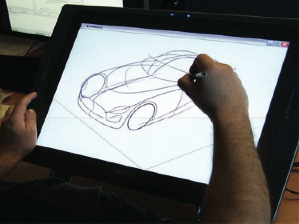
\includegraphics[width=0.7\linewidth]{gfx/baeILoveSketch}
	\caption[ILoveSketch]{ILoveSketch zeigt ein >>natürliches<< Skizziersystem, welches mehrere kaligraphische Interaktionstechniken miteinander vereint \citep{Bae:2008}.}
	\label{fig:baeILoveSketch}
	\end{center}
\end{figure}

Alvarado fasste in \citep{Alvorado:2004} eine Liste aus sieben Designguidelines zur Entwicklung von \emph{Sketch Recognition User Interfaces} (Benutzeroberflächen zur Skizzenerkennung), kurz SkRUIs zusammen: 

\begin{enumerate}
	\item Zeige Skizzenerkennungsergebnisse erst wenn der Benutzer fertig ist mit dem Zeichnen
	\item Sorge für offensichtliche Hinweise um das Skizzieren von der Erkennung zu unterscheiden
	\item Beschränke die Erkennung auf einen einzelnen Bereich, solange keine automatische Bereichserkennung machbar ist
	\item Integriere stiftbasiertes Editieren
	\item Skizzieren und Editieren sollten bestimmten Stiftbewegungen zugrunde liegen
	\item SkRUIs benötigen große Buttons
	\item Der Stift muss stets in real-time reagieren.
\end{enumerate}

Während WIMP Interfaces seit Mitte der 1980er Jahre weit verbreitet benutzt werden, müssen stiftbasierte Interfaces erst Fuß fassen. Um bessere Interaktionsrichtlinien, Interface Design Patterns und Toolkits zu entwickeln, muss die Forschung weiterhin Skizzierapplikationen entwickeln und evaluieren.

\subsection{Das Modusproblem}\label{sec:ModusProblem}
Oft interpretiert das User Interface Eingaben unterschiedlich - je nach dem in welchen Modus sich das Programm gerade befindet. Zum Beispiel hat ein Zeichenprogramm Eingabemodi wie \emph{Auswahl}, \emph{Linie zeichnen} oder \emph{Füllwerkzeug}. So ein Programm erlaubt dem Benutzer beispielsweise rechteckige Bereiche zu selektieren oder, wenn das Stifttool ausgewählt ist, zu zeichnen - beides indem der Benutzer eine Maustaste drückt und die Maus bewegt. Das Programm interpretiert die Eingaben hinsichtlich dem ausgewählten Werkzeug. \\ Manchmal ist sich der Benutzer jedoch nicht im Klaren in welchen Modus er sich befindet, oder weiß nicht wie er in einen anderen Modus umschalten kann. Die Handhabung der Modi führt oft zu kognitiver Überlastung der Benutzer, da sich diese auf das ausgewählte Tool konzentrieren anstatt auf ihre Arbeit. Dabei spricht man auch vom sog. \emph{Modusproblem} \citep{Tesler:1981}, welches seit den Anfängen interaktiver Systemen besteht und nicht nur auf Skizziersoftware beschränkt ist.

\medskip \emph{Sketchpad}\footnote{Sketchpad war ein interaktives Designsystem aus dem Jahr 1963, das Technikern erlaubte Modelle mit Hilfe eines Lichtstiftes auf einem Display zu erstellen. Der Benutzer konnte dabei verschiedene Bedingungen (wie z.B. >>erstelle eine Linie parallel zu dieser Linie und erhalte das Verhältnis) auf das Gezeichnete anwenden. \citep{Sutherland:1964}}, das wohl erste nennenswerte elektronische Skizziersystem, behalf sich mit physikalischen Steuerelementen (Knöpfe, Schalter, Regler), durch die der Benutzer mit seiner linken Hand zu den verschiedenen Modi schalten konnte (siehe \autoref{fig:ellisSketchpad}) \citep{Sutherland:1964}. 

\begin{figure}[bth]
	{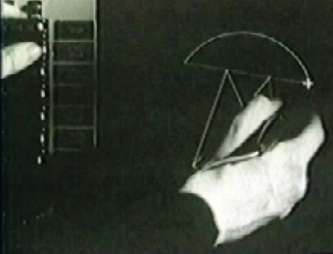
\includegraphics[width=\linewidth]{gfx/ellisSketchpad}}
	\caption[Sketchpad]{Sketchpad unterstützt Benutzer beim Erstellen von Designzeichnungen mittels Stift (rechte Hand) und verschiedener Modi/Bedingungen (erreichbar über die Knöpfe auf der linken Seite).}
	\label{fig:ellisSketchpad}
\end{figure}

\begin{figure}
        \myfloatalign
        \subfloat[Input]
        {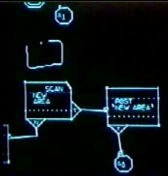
\includegraphics[width=.48\linewidth]{gfx/ellisGRAILinput}} \quad
        \subfloat[Output]
        {\label{fig:ellisGRAILinput}%
         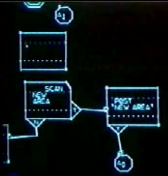
\includegraphics[width=.48\linewidth]{gfx/ellisGRAILoutput}} \\
        \caption[GRAIL Funktionalität]{GRAIL analysiert die Benutzereingaben (a) und errechnet automatisch die bestimmungsgemäße Information (b) - hier z.B. ein Rechteck.}\label{fig:ellisGRAILoutput}
\end{figure}

\medskip Im \emph{GRAIL}\footnote{RAND's GRAIL (GRAphical Input Language) System aus dem Jahr 1968, interpretierte Stifteingaben in einer besonderen visuellen Programmiersprache, um Flussdiagramme zu erstellen \citep{Ellis:1969}. Benutzer konnten via Eingabetablet semantisch wertvolle Modelldaten (Rechtecke, Pfeile, Schrift) und Kommandos (Lösche eine Linie, Bewege ein Rechteck, etc.) zeichnen und GRAIL errechnete anschließend automatisch die bestimmungsgemäße Information.} System können Benutzer nicht explizit in einen anderen Modus wechseln, um Text und Grafiken zu bearbeiten. Stattdessen versucht das System die Absichten des Benutzers aus einer Analyse des Gezeichneten bzw. dessen Kontext zu erschließen (siehe \autoref{fig:ellisGRAILoutput}) \citep{Ellis:1969}. 

\medskip Diese zwei früh entwickelten Systeme stellen zwei Extreme gegenüber, die zeigen wie man mit dem Modusproblem umgehen kann. Sketchpad's Ansatz baut auf explizite Modiwechsel abseits des Stiftes auf - GRAIL's Ansatz auf implizite Modiwechsel, errechnet durch Stifteingaben.

\medskip Es scheint keinen >>richtigen<< Weg geben, um dem Modusproblem entgegenzuwirken. Implizite Modiwechsel scheinen natürlicher, aber nur wenn das System die Benutzereingaben richtig interpretiert. Interpretationstechniken sind fehleranfällig. Viele Systeme ermöglichen deswegen eine Kombination dieser zwei Arten oder verhängen Zeichenkonventionen.

\medskip Saund and Lank erforschten automatische Interpretationen und Modiwechsel, basierend auf Eingaben von Benutzern und bereits Gezeichneten \citep{Saund:2003p66}. Ihr \emph{Inferred-Mode Protocol} beschreibt einen Ansatz zur Analyse des Gezeichneten, um herauszufinden ob Aktionen mit Absicht durchgeführt wurden, oder nicht. War eine Aktion unklar, wird ein Mediator eingesetzt, der Methoden vorschlägt, um die Unklarheit zu beseitigen.

\medskip Li et al. verglichen in \citep{Li:2005} verschiedene Moduswechseltechniken für stiftbasierende User Interfaces. Dabei wurden folgende Techniken miteinbezogen: 
\begin{itemize}
	\item Tasten am Stift,
	\item Drücken und Halten,
	\item Benutzung der Hilfshand um einen physikalischen Button zu drücken,
	\item ein neue durckbasierte Methode, und
	\item Benutzung des >>Radierers<< des Stiftes
\end{itemize}

Interessanterweise, war die Methode, in der die Hilfshand verwendet wurde die schnellste, am Fehler unanfälligsten und die beliebteste. Die >>Drücken und Halten<< Methode, wurde auch von Schilit et al. \citep{Schilit:1998} verwendet, die dies auch >>Rast<<-Geste bezeichneten. Microsoft Windows for Tablet PCs benutzt diese Geste beispielsweise um die Rechtsklick-Kontextmenüs aufzurufen.

\medskip Bei Skizziersystemen tritt das Modusproblem vorwiegend auf, da es mehrere Typen an Stifteingaben gibt. Manche Eingaben sollen auf einer Seite angezeigt werden, da sie Wörter, Zeichnungen oder andere Modellelemente (\emph{Model Operations}) darstellen, andere sollen im Hintergrund weiterverarbeitet werden, da sie Selektionen oder Kommandos (\emph{Environment Operations}) angeben.

\medskip \emph{Flow Selection} \citep{Johnson:2006} erlaubt Benutzern mit Hilfe der Rast-Geste nahtlos vom Zeichen- zum Selektionsmodus zu wechseln. Anschließende Operationen, wie Verschieben eines Teilabschnitts einer Linie, werden durch Bewegung des Stiftes ausgeführt -- ohne den Stift vorher abzusetzen. Wieviel Einzelpunkte vom darunter liegenden Objekt selektiert werden - man spricht dabei auch von der Selektionstärke - hängt vom Abstand zur Stiftposition ab und wie lange der Benutzer den Stift an der selben Stelle ruhen lässt. Die Selektionstärek wird bei Operationen wie Verschieben oder Glättung verwendet (vgl. \autoref{fig:johnsonFlowSelection2}).

\begin{figure}
        \myfloatalign
        \subfloat[ ]
        {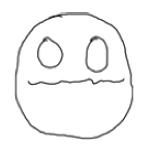
\includegraphics[width=.22\linewidth]{gfx/johnsonFlowSelection1}} \quad
        \subfloat[ ]
        {\label{fig:johnsonFlowSelection1}%
         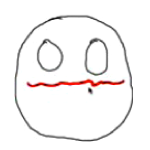
\includegraphics[width=.22\linewidth]{gfx/johnsonFlowSelection2}} \quad
		\subfloat[ ]
        {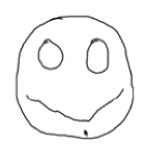
\includegraphics[width=.22\linewidth]{gfx/johnsonFlowSelection3}} \quad
        \subfloat[ ]
        {\label{fig:johnsonFlowSelection1}%
         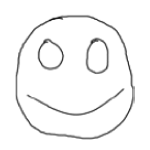
\includegraphics[width=.22\linewidth]{gfx/johnsonFlowSelection4}} \quad
        \caption[Modiwechsel]{Modiwechsel der Flow Selection geschehen durch Halten und Bewegen des Stiftes \citep{Johnson:2006}. Der Benutzer positioniert dazu den Stift am gewünschten Objekt (a), bewegt es (b) ohne dabei den Stift zu heben (c). Der Benutzer hält den Stift anschließend an der Position bis die Kurve geglättet wurde (d) bevor er den Prozess durch heben des Stiftes abschließt.}\label{fig:johnsonFlowSelection2}
\end{figure}

\section{Mixed Reality}

\section{Die Bedeutung von Gestik}

\begin{quote}
	\begin{flushright}{\slshape    
	    Design is an “activity of the mind \ldots grounded in mechanisms that evolved for interaction with the environment”.} \\ \medskip
	    --- \defcitealias{Wilson:2002}{M. Wilson}\citetalias{Wilson:2002} \citep{Wilson:2002}
	\end{flushright}
\end{quote}

Die Kombination von Gesten und Sprache bilden die Grundlage zur menschlichen dialogorientierten Interaktion. Um diese Modalitäten auch richtig in HCI\footnote{Human Computer Interaction (HCI) oder dt. Mensch-Computer-Interaktion ist ein Teilgebiet der Informatik und beschäftigt sich mit der benutzergerechten Gestaltung von Systemen.} anwenden zu können, müssen wir ihre Wechselwirkung \ldots

Die Benutzung von Gesten in Verbindung mit Skizzen ermöglicht es Meetingteilnehmer Details zu einer vorliegenden Arbeit zu erklären und zu interpretieren. Zusätzlich können hypothetische Modifikationen vorgenommen werden. Gesten bieten einen Mechanismus um Aktivitäten, Größen, Verbindungen, Richtungen oder Blickrichtungen zu kommunizieren. 
\\ Dantec schildert in \citep{Dantec:2009} die Erfahrungen, die er in einem Architekturdesignmeeting mit Gestik gemacht hat. Über das gesamte Meeting hinweg waren Gesten das primäre Mittel um Designprobleme zu lösen. Trotz der unbeständigen Natur von Gesten, wurden sie wiederholt und effektiv eingesetzt um komplexe Konzepte zu kommunizieren, ohne zuvor ein spezielles Training absolviert zu haben. Die Wirksamkeit von Gesten und die Art wie sie zwischen allen Teilnehmer fungierten, zeigte wie mehrere Teilnehmer mit eigenen Spezialisierungen ein verständliches Kommunikationsmittel fanden und so zum gemeinsamen Design beitrugen.
%\\ Wilson beschrieb , dass Design >>Gedankenarbeit [ist,] ... die mit Mechanismen, die sich zur Interaktion mit der Umwelt entwickelten, verankert ist<< \citep{Wilson:2002}.

\medskip In Dantecs beschriebenen Szenario wurden Gesten auch dazu verwendet, um über Merkmale von Designs zu sprechen, die im zweidimensionalen Design nicht eindeutig hervorgingen. So machte z.B. ein Teilnehmer große schwungvolle Gesten um die Form und Platzierung kleiner Fenster in einer Kapelle zu beschreiben (siehe \autoref{fig:dantecGestures}). Die Gesten zeigten mit der Hilfe von den Skizzen ein klares Bild von Form und Größe, boten zudem aber noch mehr. Sie beinhalteten eine metaphorische Qualität, da sie ausdrücken konnten wie der Raum Ruhe erzeugt. Somit bekräftigten sie den Zweck des Gebäudes, der als Ort der Trauer gilt (siehe \extref{ext:dantecGestures}). Die Tatsache, dass die Nutzung von Gesten, physikalische Eigenschaften und metaphorische Qualitäten beschreiben kann, bestätigen auch die Forschungsergebnisse von Casasanto und Lozano, die die Rolle von Gesten beim Erarbeiten von abstrakten Konzepten untersuchten \citep{Casasanto:2006}.

\begin{figure}[bth]
	{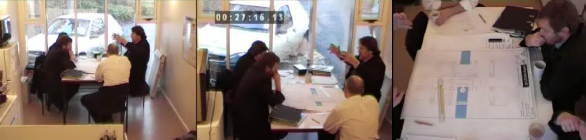
\includegraphics[width=\linewidth]{gfx/dantecGestures}}
	\caption[Gestures]{Ein Teilnehmer gestikuliert um Gebäudemerkmale zu beschreiben.}
	\label{fig:dantecGestures}
\end{figure}

\begin{extract}[Transkript eines Designmeetings. Skizzen und Gestik dienen als Ausdrucksmittel.]{
		\myfloatalign
		\begin{tabularx}{\textwidth}{p{1cm}X}
    		Adam & that wasn’t the idea I was anticipating that the hearses would be parked here [sketches] \\
			Anna & were there OK that’s fine yeah \\
			Adam & exactly as they are at the moment that the coffin would be drawn out	here and they would simply [points] walk it in I wasn’t thinking that they’d try and park \\
			Anna & no that’s OK \\
			Adam & in there \\
			Anna & yes well that’s what they’re wondering how that would work then so we’d work I wasn’t quite aware \\
			Adam & we’d work it exactly the same way as the present system I mean maybe this should be made more obvious by perhaps a different colour in the paving or something [sketches] I mean what I’m trying to say here is that that’s the vehicular line [sketches] \\
			Anna & yes \\
			Adam & and that these areas [points] are for people to mill about in and you’ve got a place for people to stand \\
			Anna & yes they will probably want to know how [points] how + how far that is from the because they’re going to be possibly carry the coffins in and most of the men are sort of in their seventies and eighties [laughs] carrying the coffin \\
		\end{tabularx}
	}
	\label{ext:dantecGestures}
\end{extract}


\section{Case Study - Digital and Paper Media}

\section*{Zusammenfassung}
lorem ipsum